            \begin{question}{1207}{Nombres complexes}{1}{1223}
                Dans quelle partie du plan complexe se situe $2-5i$?
            \end{question}
            \begin{reponses}
                \item[false] En haut à droite.
                \item[true] En bas à droite.
                \item[false] En bas à gauche.
                \item[false] En haut à gauche.
            \end{reponses}
            %%%%%%%%%%%%%%%%%%%%%%%%%%%%%%%%%%%%%
            \begin{question}{1207}{Nombres complexes}{2}{1223}
                Comment s'écrit le nombre complexe $A$?\\
                \begin{center}
                	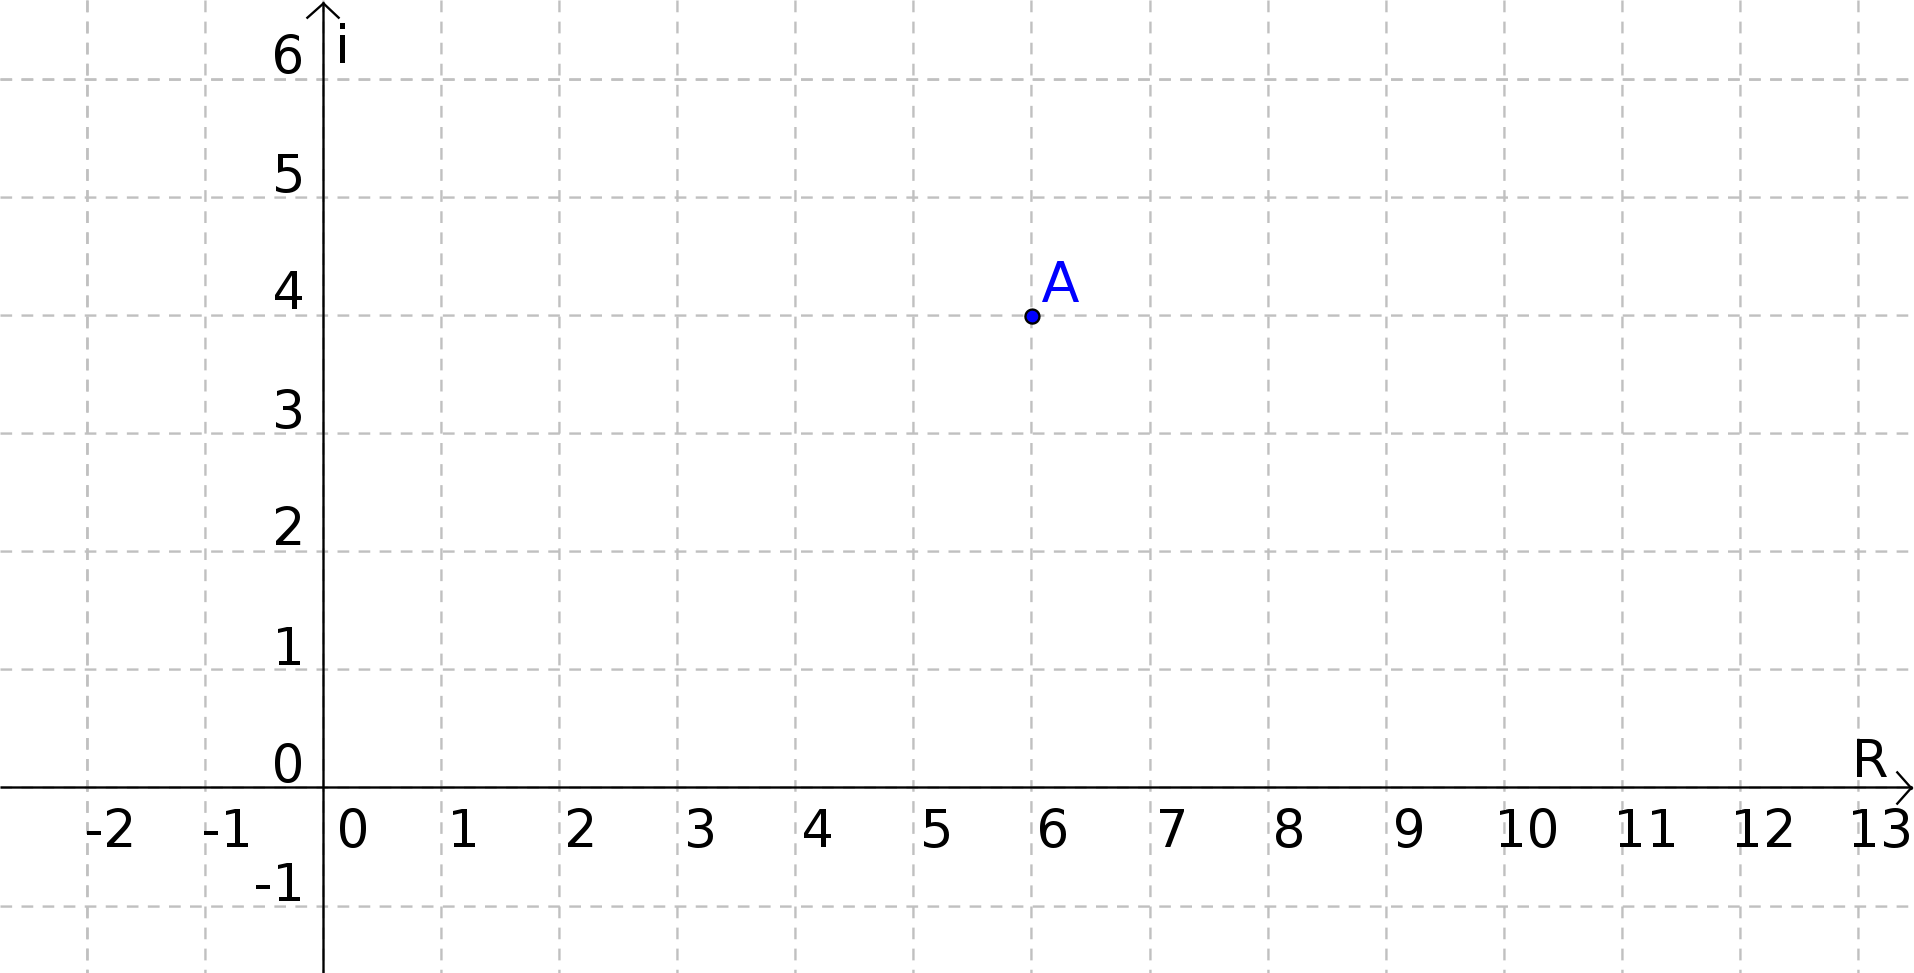
\includegraphics[width=0.5\textwidth]{Philippe/Figures_Philippe/complexes_5_1.png}
                \end{center}
            \end{question}
            \begin{reponses}
                \item[false] $6-4i$
                \item[false] $4+6i$
                \item[true] $6+4i$
                \item[false] $4-6i$
            \end{reponses}
            %%%%%%%%%%%%%%%%%%%%%%%%%%%%%%%%%%%%%
            \begin{question}{1207}{Nombres complexes}{1}{1223}
                L'impédance d'un système électrique de partie résistive $R$ et de partie réactive $X$ est $Z = R + iX$, avec $i^2=-1$. Dans quelle partie du plan complexe se situe $Z$ si $R=-2$ et $X=4$?
            \end{question}
            \begin{reponses}
                \item[false] En haut à droite.
                \item[false] En bas à droite.
                \item[false] En bas à gauche.
                \item[true] En haut à gauche.
            \end{reponses}
            %%%%%%%%%%%%%%%%%%%%%%%%%%%%%%%%%%%%%
